\begin{titlepage}

\newcommand{\HRule}{\rule{\linewidth}{0.5mm}}
% \renewcommand{\baselinestretch}{2.0}
\centering

\large ĐẠI HỌC QUỐC GIA THÀNH PHỐ HỒ CHÍ MINH \\
TRƯỜNG ĐẠI HỌC BÁCH KHOA \\
KHOA ĐIỆN - ĐIỆN TỬ  \\
BỘ MÔN VIỄN THÔNG  \\ [0.8cm]

\begin{figure}[!ht]
    \centering
    
\includegraphics[scale=0.3]{front_pages/Logo_BK.png}
    \label{fig:logo}
\end{figure}

\bfseries
\Large{LUẬN VĂN TỐT NGHIỆP ĐẠI HỌC} \\[1.3cm]

\LARGE{NHẬN DẠNG NGÔN NGỮ KÝ HIỆU CHO NGƯỜI KHIẾM THÍNH SỬ DỤNG KỸ THUẬT HỌC SÂU: TÁCH VÀ PHÂN TÍCH ĐẶC TRƯNG KHUNG XƯƠNG TRÊN VIDEO RGB} \\ [2.1cm]

\normalfont
\normalsize
% \small
\begin{tabular}{r l}
    \fontsize{14pt}{0pt}{\selectfont{GVHD:}} & \fontsize{14pt}{0pt}{\selectfont{PGS.TS HÀ HOÀNG KHA}} \\
    \fontsize{14pt}{0pt}{\selectfont{SVTH:}} & \fontsize{14pt}{0pt}{\selectfont{NGUYỄN THÀNH ĐẠT - 1510698}}  					
                        
\end{tabular} 
\\ [2.1cm]

TP. HỒ CHÍ MINH, THÁNG 12 NĂM 2019
% \vfill
\end{titlepage}


%------------------------------------------------------------------
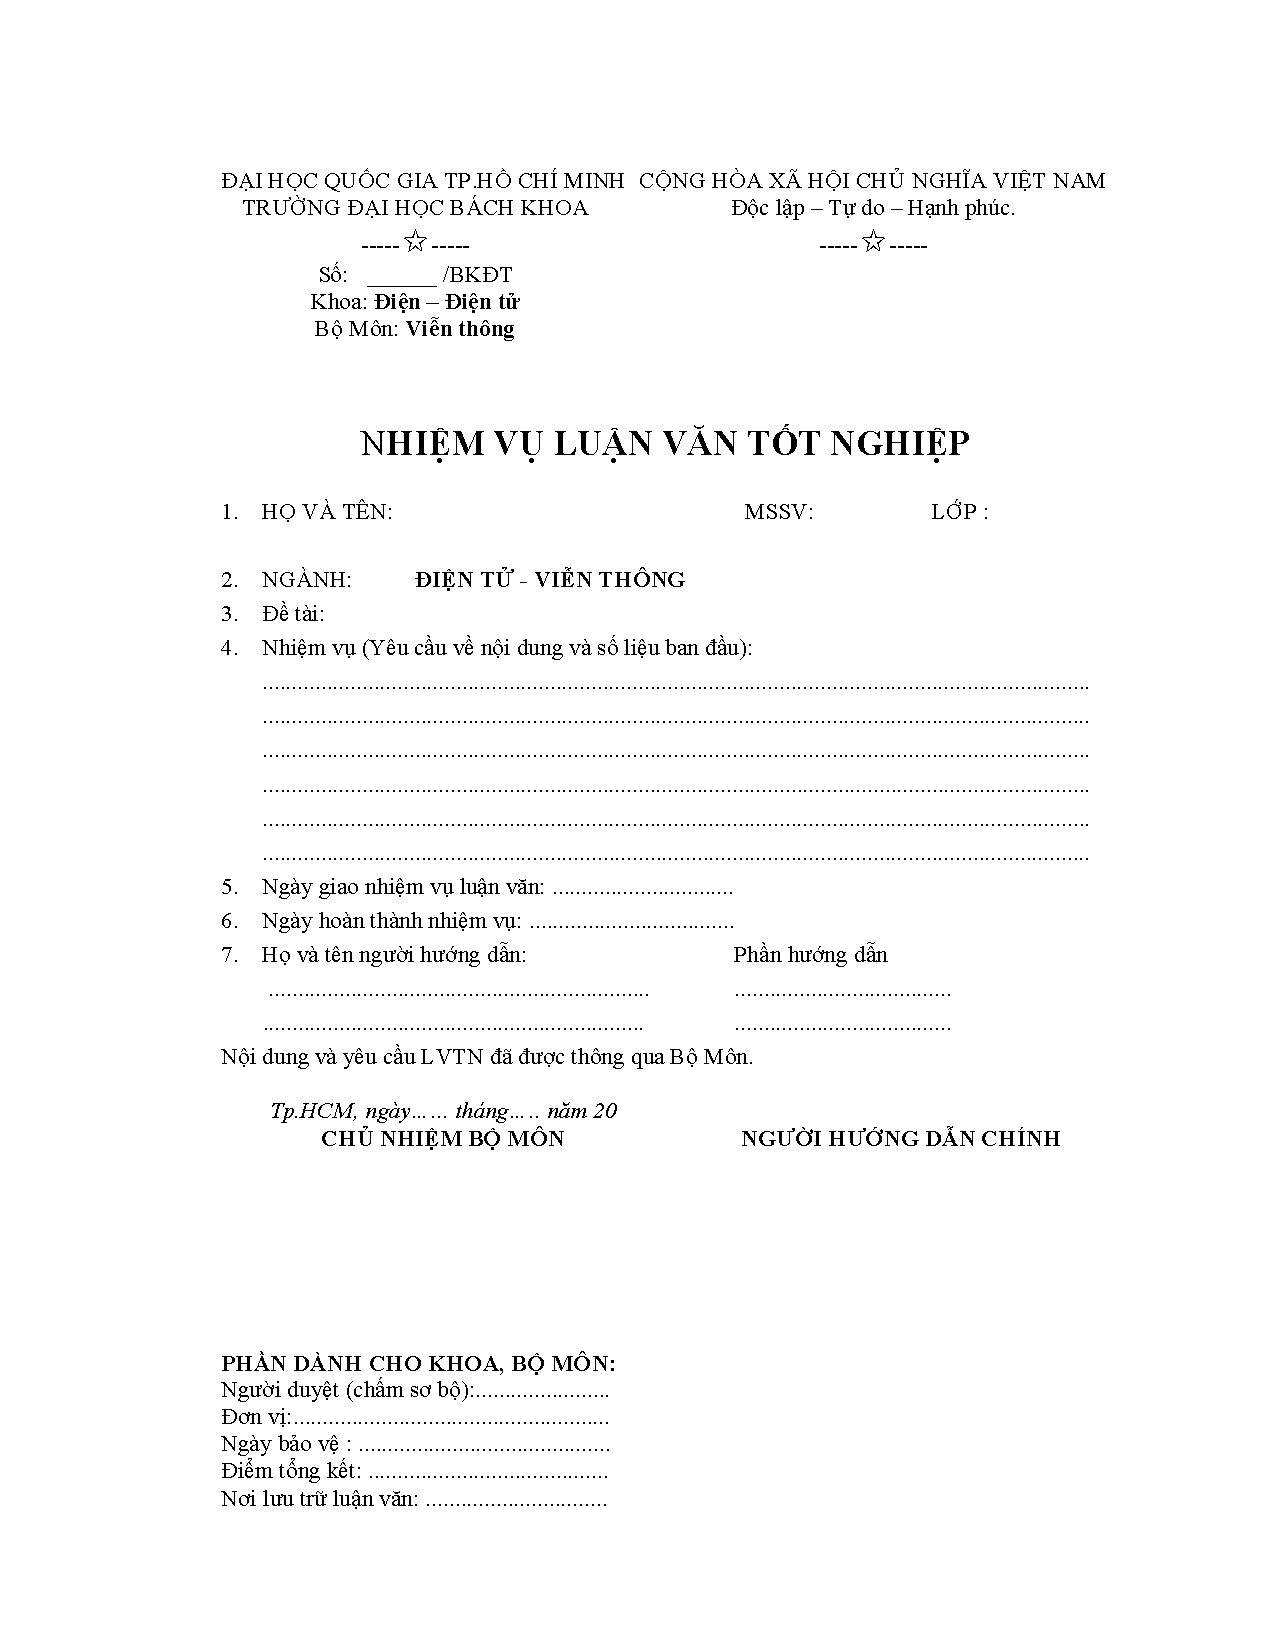
\includepdf[pages=-]{front_pages/nhiem_vu_lv.pdf}

%------------------------------------------------------------------
\newpage
\pagenumbering{roman}
\addcontentsline{toc}{chapter}{LỜI CẢM ƠN}
\thispagestyle{loi_cam_on}
\begin{center}
{\fontsize{18pt}{30pt}{\selectfont{\textbf{Lời cảm ơn}}}}
\end{center}

\textit{Trong thời gian thực hiện luận án này, em đã nhận được sự hỗ trợ nhiệt tình, hướng dẫn tận tình và những lời động viên tích cực từ các giảng viên, bạn bè và gia đình. Do đó, em đã hoàn thành luận án như mục tiêu đã đặt ra. Những lời giảng dạy quý báu, không những về mặt kiến thức mà còn về đạo đức làm người của các quý thầy cô sẽ là hành trang cho con đường tương lai của các thế hệ sinh viên.}

\textit{Em xin gửi đến thầy Hà Hoàng Kha, giảng viên hướng dẫn trực tiếp đề tài, lời biết ơn sâu sắc. Thầy đã dành thời gian quý báu để gặp gỡ, thảo luận, đưa ra những vấn đề hay để rèn luyện chúng tôi khả năng giải quyết vấn đề. Thầy là người đã theo tường bước đi của chúng tôi, tận tình chỉ bảo, hướng dẫn chúng tôi từ khi làm đồ án, đề cương cho đến luận văn. Ngoài những kiến thức chuyên ngành, chúng tôi còn nhận được những lời khuyên, kinh nghiệm quý giá trong học tập và nghiên cứu từ thầy.}

\textit{Em cũng xin cảm ơn chân thành đến cha mẹ đã động viên và tạo điều kiện giúp đỡ chúng tôi vượt qua những khó khăn trong suốt quá trình học tập và nghiên cứu.}

\textit{Mặc dù đã cố gắng trong phạm vi và khả năng cho phép, nhưng luận văn không thể tránh khỏi những thiếu sót, rất mong được sự góp ý của quý thầy cô và các bạn.}

\textit{Cuối cùng, xin chân thành cảm ơn quý thầy cô và các bạn đã dành thời gian đọc luận văn này.}


%------------------------------------------------------------------
\newpage
\addcontentsline{toc}{chapter}{LỜI CAM ĐOAN}
\thispagestyle{loi_cam_doan}
\begin{center}
{\fontsize{18pt}{30pt}{\selectfont{\textbf{Lời cam đoan}}}}
\end{center}

\noindent Em xin cam đoan rằng, luận văn tốt nghiệp "Nhận dạng ngôn ngữ ký hiệu cho người khiếm thính sử dụng kỹ thuật học sâu: tách và phân tích đặc trưng khung xương trên video RGB" là công trình nghiên cứu của em dưới sự hướng dẫn của PGS.TS Hà Hoàng Kha. Đề tài xuất phát từ nhu cầu thực tiễn và nguyện vọng muốn thực hiện của em. Ngoại trừ những nội dung được biên soạn lại từ các công trình khác đã ghi rõ, các nội dung, kết quả kiểm tra đánh giá thực nghiệm trình bày trong luận văn này là kết quả nghiên cứu do chính em thực hiện, hoàn toàn không phải sao chép từ bất kỳ một tài liệu hoặc công trình nghiên cứu nào khác.

Nếu không thực hiện đúng các cam kết trên, chúng tôi xin hoàn toàn chịu trách nhiệm trước kỷ luật của nhà trường cũng như pháp luật Nhà nước.

\begin{flushright}
Sinh viên thực hiện
\end{flushright}


%------------------------------------------------------------------
\newpage
\addcontentsline{toc}{chapter}{TÓM TẮT}
\thispagestyle{tom_tat}
\begin{center}
{\fontsize{18pt}{30pt}{\selectfont{\textbf{Tóm tắt}}}}
\end{center}

Trong luận văn này, em đã thực hiện viết ứng dụng realtime nhận diện được một số từ ngữ thông dụng trong ngôn ngữ ký hiệu của người khiếm thính khi giao tiếp. Ứng dụng được xây dựng với mục đích giúp cho người khiếm thính giao tiếp dễ dàng hơn với người bình thường khi họ không hiếu ngôn ngữ ký hiệu của người khiếm thính.

Bởi những phát triển trong học máy và học sâu gần đây, đã giúp con người giải quyết được những bài toán thực tế mà trước đây tưởng chừng như máy tính không thể làm được. Trong ứng dụng này em đã sử dụng một trong các phương pháp học máy đó để giải quyết bài toán nhận diện ngôn ngữ ký hiệu cho người khiếm thính Việt Nam. Phương pháp nhận diện mà đề tài sử dụng chia làm 2 bước. Đầu tiên từ hình ảnh RGB có chứa hình ảnh người khiếm thính đang diễn tả một từ ngữ do camera truyền vào. Ứng dụng sử dụng một mạng CNN là mạng mobilenet để trích xuất đặc trưng khung xương là tọa độ các khớp xương trên ảnh 2D (tổng cộng có 18 khớp xương ban đầu). Sau đó các tọa độ khớp xương này được đưa vào một mạng DNN để từ đó phân loại ra các hành động diễn tả từ ngữ mà mạng đã học được. Cuối cùng ứng dụng xuất ra từ ngữ mà người đứng trước camera muốn diễn tả và xuất ra màn hình.

Phương pháp nhận diện dựa vào trích xuất đặc trưng khung xương là một phương pháp khá hay và lạ so với các nghiên cứu liên quan trước đây. Điểm hay của phương pháp này là việc trích xuất khung xương đã khái quát gần như toàn bộ tư thế và hành động mà người khiếm thị muốn diễn tả. Việc này còn làm giảm số chiều dữ liệu so với việc từ một hình ảnh RGB đưa vào để phân loại ra từ ngữ gì. Việc còn lại chỉ cần phân loại hành động dựa trên đặc trưng đã được trích xuất bằng một mạng DNN cấu trúc nhỏ. Việc này giúp tăng tốc độ xử lý của ứng dụng lên đáp ứng được việc xử lý realtime.

Các kết quả thực nghiệm thu được từ hệ thống cho thấy tỷ lệ nhận dạng cao và tốc độ đáp ứng đủ nhanh cho hoạt động chế độ thời gian thực.

%------------------------------------------------------------------
\newpage
\thispagestyle{abstract}
\begin{center}
{\fontsize{18pt}{30pt}{\selectfont{\textbf{ABSTRACT}}}}
\end{center}



\textbf{Key words:} 

%------------------------------------------------------------------
\newpage
\addcontentsline{toc}{chapter}{MỤC LỤC}
{\fontsize{12pt}{5pt}\selectfont
\tableofcontents}


%------------------------------------------------------------------
\newpage
\addcontentsline{toc}{chapter}{DANH SÁCH HÌNH VẼ}
\listoffigures


%------------------------------------------------------------------
\newpage
\addcontentsline{toc}{chapter}{DANH SÁCH BẢNG}
\listoftables


%------------------------------------------------------------------
\newpage
\thispagestyle{danhmucviettat}
\addcontentsline{toc}{chapter}{DANH MỤC VIẾT TẮT}
{\fontsize{18pt}{30pt}{\selectfont{\textbf{Danh mục viết tắt}}}}

\FloatBarrier
\begin{table}[h]
\centering
\captionsetup{list=no}
\begin{center}
\begin{tabularx}{\columnwidth}{XX}
NN & : Neural Network \\
CNNs & : Convolutional Neural Networks\\
DNN & : Deep Neural Network \\
DL & : Deep Learning \\
MLP & : Multi Layer Perceptron \\
SGD & : Stochastic Gradient Descent \\
SJM & : Skeleton Joints Mapping \\
PAFs & : Part Affinity Fields  \\
CFMs & : Confidence Maps

\end{tabularx}
\end{center}
\end{table}
\FloatBarrier